%
%  cel-lsy-6
%
\tikzsetnextfilename{figures/triplet/triplet}
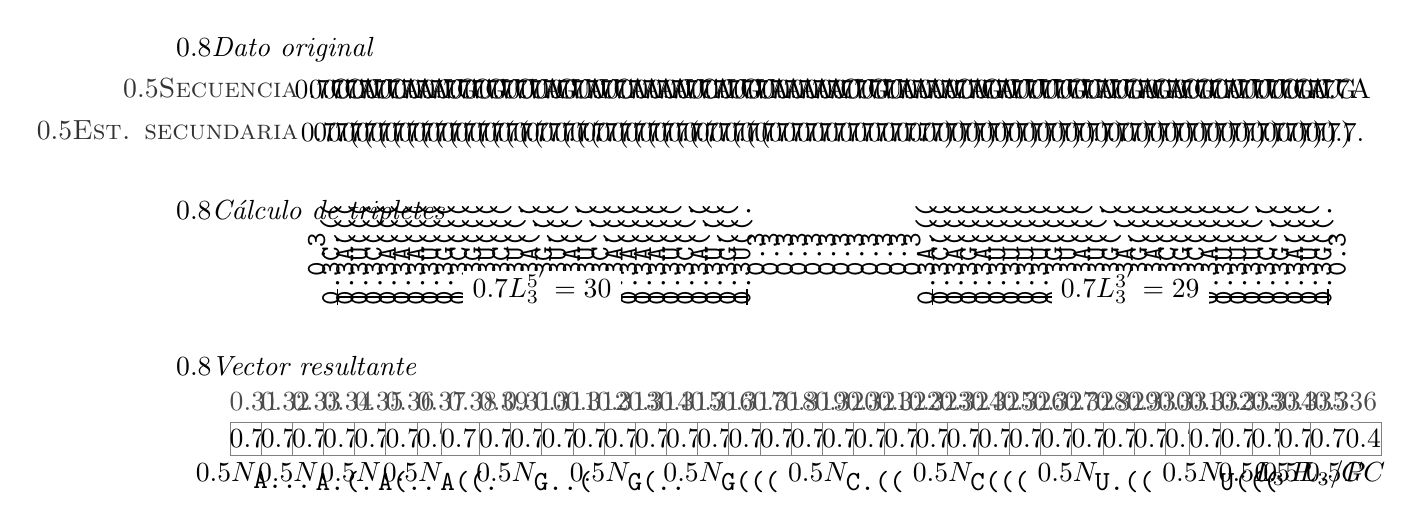
\begin{tikzpicture}[
  scale=0.18,
  every node/.style={
    anchor=base,
  }
]
  %
  \tikzstyle{tit}=[
    anchor=base west,
    font=\relscale{0.8}\itshape,
    %black!80,
  ];
  \tikzstyle{etiqueta}=[
    anchor=base east,
    font=\relscale{0.5}\scshape,
    black!80,
    yshift=0.5,
  ];
  \node[tit] () at (-10,7)   {Dato original};
  \node[tit] () at (-10,-4.5)  {Cálculo de tripletes};
  \node[tit] () at (-10,-15.5) {Vector resultante};

  %
  \node[etiqueta] () at (-0,4)  {Secuencia};
  \node[etiqueta] () at (-0,1)  {Est. secundaria};

  %%%%%%%%%%%%%%%%%%%%%%%%%%%%%%%%%%%%%%%%%%%%%%%%%%%%%%%%%%%%%%%%%%%%
  
  % generate \foreach sequence with:
  %>>> seqn = 'CCAUCAAAUGCGUCUAGUAUCAAAAUCAUGUAAAAACUGUAAAACAGAUUUUGUAUGAGACGCAUUUCGAUGA'
  %>>> stru = '.((((((((((((((.(((.(((((((.(((............))))))))))))).)))))))))).)))).'
  %>>> stru = '.' + stru + '.'
  %>>> iter = ''
  %>>> for i in range(len(seqn)):
  %...     iter = iter + seqn[i] + ' / {' + stru[i+1] + '} / {' + seqn[i] + stru[i:i+3].replace(')','(') + '} , '
  %... 
  %>>> iter
  \foreach \q/\t/\3 [count=\c] in {
    C / {.} / {} , C / {(} / {C.((} , A / {(} / {A(((} , U / {(} / {U(((}
    , C / {(} / {C(((} , A / {(} / {A(((} , A / {(} / {A(((} , A / {(} /
    {A(((} , U / {(} / {U(((} , G / {(} / {G(((} , C / {(} / {C(((} , G /
    {(} / {G(((} , U / {(} / {U(((} , C / {(} / {C(((} , U / {(} / {U((.}
    , A / {.} / {A(.(} , G / {(} / {G.((} , U / {(} / {U(((} , A / {(} /
    {A((.} , U / {.} / {U(.(} , C / {(} / {C.((} , A / {(} / {A(((} , A /
    {(} / {A(((} , A / {(} / {A(((} , A / {(} / {A(((} , U / {(} / {U(((}
    , C / {(} / {C((.} , A / {.} / {A(.(} , U / {(} / {U.((} , G / {(} /
    {G(((} , U / {(} / {U((.} , A / {.} / {} , A / {.} / {} , A / {.} / {}
    , A / {.} / {} , A / {.} / {} , C / {.} / {} , U / {.} / {} , G / {.}
    / {} , U / {.} / {} , A / {.} / {} , A / {.} / {} , A / {.} / {} , A /
    {)} / {A.((} , C / {)} / {C(((} , A / {)} / {A(((} , G / {)} / {G(((}
    , A / {)} / {A(((} , U / {)} / {U(((} , U / {)} / {U(((} , U / {)} /
    {U(((} , U / {)} / {U(((} , G / {)} / {G(((} , U / {)} / {U(((} , A /
    {)} / {A(((} , U / {)} / {U((.} , G / {.} / {G(.(} , A / {)} / {A.((}
    , G / {)} / {G(((} , A / {)} / {A(((} , C / {)} / {C(((} , G / {)} /
    {G(((} , C / {)} / {C(((} , A / {)} / {A(((} , U / {)} / {U(((} , U /
    {)} / {U(((} , U / {)} / {U((.} , C / {.} / {C(.(} , G / {)} / {G.((}
    , A / {)} / {A(((} , U / {)} / {U(((} , G / {)} / {G((.} , A / {.} /
    {}
  } {
    \coordinate[] (top\c) at (\c,8);
    \coordinate[] (low\c) at (\c,-10);
    
    \node[anchor=base,font=\relscale{0.7}] (ns\c) at (\c,4) {\q};

    \coordinate[] (str\c) at (\c,1);
    \node[anchor=base,font=\relscale{0.7}] (n2\c) at (\c,1) {\t};

    \coordinate[] (tr\c) at (\c,-5 );
    \node[anchor=base,font=\ttfamily\relscale{0.3},rotate=90,yshift=-1] (n3\c) at (\c,-7) {\3};
  }

  \tikzstyle{cota}=[
    midway,
    fill=white,
    font=\relscale{0.7},
    inner ysep=0,
  ];
  
  \draw[|-|] (low2) -- (low31) node [cota] {$L_3^{5'}=30$};
  \draw[|-|] (low44) -- (low72) node [cota] {$L_3^{3'}=29$};

  %%%%%%%%%%%%%%%%%%%%%%%%%%%%%%%%%%%%%%%%%%%%%%%%%%%%%%%%%%%%%%%%%%%%
  
  \usetikzlibrary{shapes.geometric}
  \usetikzlibrary{positioning}
  
  \tikzstyle{vec}=[
    draw=black!50,
    anchor=center,
    inner sep=0,
    minimum height=12,
    minimum width=12,
    ultra thin,
    fill=white,
    font=\relscale{0.7},
  ];
  \tikzstyle{vidx}=[
    font=\relscale{0.3},
    black!70,    
  ];
  \foreach \c / \v in {
     1/0, 2/0, 3/0, 4/2, 5/0, 6/2, 7/1, 8/14,
     9/0, 10/0, 11/0, 12/2, 13/0, 14/1, 15/2, 16/7,
    17/0, 18/0, 19/0, 20/1, 21/0, 22/1, 23/2, 24/5,
    25/0, 26/0, 27/0, 28/1, 29/0, 30/1, 31/4, 32/14,
    33/59, 34/27, 35/2.2, 36/0.4
  } {
      \pgfmathsetmacro\cpos{ \c * 2.2 - 6 };
      \node[vidx] (n\c) at (\cpos,-18) {\c};
      \node[vec] () at (\cpos,-20) {$\v$};
      \coordinate (sub\c) at (\cpos,-23);
  }

  \tikzstyle{sub} = [
    font=\relscale{0.5},
  ];
  
  \node[sub] () at (sub1) {$N_{\texttt{A...}}$};
  \node[sub] () at (sub3) {$N_{\texttt{A.(.}}$};
  \node[sub] () at (sub5) {$N_{\texttt{A(..}}$};
  \node[sub] () at (sub7) {$N_{\texttt{A((.}}$};
  \node[sub] () at (sub10) {$N_{\texttt{G..(}}$};
  \node[sub] () at (sub13) {$N_{\texttt{G(..}}$};
  \node[sub] () at (sub16) {$N_{\texttt{G(((}}$};
  \node[sub] () at (sub20) {$N_{\texttt{C.((}}$};
  \node[sub] () at (sub24) {$N_{\texttt{C(((}}$};
  \node[sub] () at (sub28) {$N_{\texttt{U.((}}$};
  \node[sub] () at (sub32) {$N_{\texttt{U(((}}$};
  \node[sub] () at (sub33) {$L_3$};
  \node[sub] () at (sub34) {$P$};
  \node[sub] () at (sub35) {$L_3/P$};
  \node[sub] () at (sub36) {$GC$};
  %
\end{tikzpicture}
